\documentclass[../notes.tex]{subfiles}

\pagestyle{main}
\renewcommand{\chaptermark}[1]{\markboth{\chaptername\ \thechapter\ (#1)}{}}
\stepcounter{chapter}

\begin{document}




\chapter{Group Theory Foundations}
\section{Groups of Low Order}
\begin{itemize}
    \item \marginnote{10/3:}Calegari: Nothing in particular to know for missing Friday; Adi will get me notes.
    \item Having explored examples, today, we're coming back down to earth to flex our axiomatic muscles.
    \item Distinguishing sets and binary operations.
    \begin{table}[h!]
        \centering
        \small
        \renewcommand{\arraystretch}{1.2}
        \begin{tabular}{c|c|c|c}
            Group & $G$ & $*$ & ?\\
            \hline
            $S_n$ & shuffles & composition & cards\\
            $\text{O}(n)$ and $\text{SO}(n)$ & (sp) orthogonal matrices & composition & vectors?\\
            $\Z$ & integers & addition\\
            $\Z/n\Z$ & $\{0,1,\dots,n-1\}$ & addition modulo $n$
        \end{tabular}
        \caption{Elements of a group.}
        \label{tab:setsBinaryops}
    \end{table}
    \begin{itemize}
        \item Be careful not to confuse the shuffles and the cards; the cards are something else curious but are \emph{not} the elements of the group.
        \item Notice that $\Z$ and $\Z/n\Z$ are \textbf{commutative} groups, but the shuffles (for $n>1$) and $\text{O}(n)$ are not.
        \item Note that $S_2$, $\text{O}(1)$, and $\Z/2\Z$ are all isomorphic groups.
    \end{itemize}
    \item \textbf{Commutative} (group): A group such that for all $x,y\in G$, $x*y=y*x$. \emph{Also known as} \textbf{Abelian}.
    \item Lemma (Cancellation Lemma): Let $x,y,z\in G$. Then $xy=xz$ implies $y=z$ and $yx=zx$ implies $y=z$.
    \begin{proof}
        We have that
        \begin{align*}
            x*y &= x*z\\
            x^{-1}*(x*y) &= x^{-1}*(x*z)\tag*{Inverses exist}\\
            (x^{-1}*x)*y &= (x^{-1}*x)*z\tag*{Associativity}\\
            e*y &= e*z\\
            y &= z
        \end{align*}
        as desired.\par
        The proof of the second statement is symmetric.
    \end{proof}
    \begin{itemize}
        \item This will be Calegari's only proof from the axioms directly.
    \end{itemize}
    \item \textbf{Multiplication table} (for $G$): A table with all elements of $G$ on the top and the side, and all binary products in it.
    \begin{itemize}
        \item The total number of binary operations is $n^{n^2}$?
        \item To check that a group is a group, we can write out its multiplication table and confirm pointwise that the group axioms are satisfied. However, there are also many ways to speed this process up.
        \item An example of a multiplication table can be found on the right in Figure \ref{fig:Sudoku3}.
    \end{itemize}
    \item \textbf{Trivial group}: The only group with $|G|=1$, i.e., $G=\{e\}$.
    \item A group of $|G|=2$ has the form $G=\{e,x\}$ where we must have $x=x^{-1}$.
    \begin{itemize}
        \item We can find this by inspection or invoke the \textbf{Sudoku Lemma}.
        \item Thus, all groups of order 2 are isomorphic.
    \end{itemize}
    \item Lemma (Sudoku Lemma): Fix $x\in G$. Then
    \begin{equation*}
        \{xg\mid g\in G\} = G
        = \{gx\mid g\in G\}
    \end{equation*}
    \begin{proof}
        There exists $g$ such that $xg=y$ for $x,y$ fixed: Choose $g=x^{-1}y$.\par
        $y$ only occurs once: If $xg=y$ and $xg'=y$, transitivity and the cancellation lemma imply $g=g'$.
    \end{proof}
    \begin{itemize}
        \item In layman's terms, in every row and column of the multiplication table, each element of $G$ occurs exactly once.
    \end{itemize}
    \item Playing Sudoku, we can show that all groups of order 3 are isomorphic.
    \begin{figure}[h!]
        \centering
        \small
        \renewcommand{\arraystretch}{1.2}
        \begin{tikzpicture}
            \node at (-2.5,0) {
                \begin{tabu}{c|[0.8pt]c|c|c}
                     & \multicolumn{1}{c}{$e$} & \multicolumn{1}{c}{$x$} & $y$\\
                    \tabucline[1pt]{-}
                    $e$ & $e$ & $x$ & $y$\\
                    \tabucline{2-}
                    $x$ & $x$ &  & \\
                    \tabucline{2-}
                    $y$ & $y$ &  & \\
                \end{tabu}
            };
            \draw [-stealth] (-0.4,0) -- (0.4,0);
            \node at (2.5,0) {
                \begin{tabu}{c|[0.8pt]c|c|c}
                     & \multicolumn{1}{c}{$e$} & \multicolumn{1}{c}{$x$} & $y$\\
                    \tabucline[1pt]{-}
                    $e$ & $e$ & $x$ & $y$\\
                    \tabucline{2-}
                    $x$ & $x$ & $y$ & $e$\\
                    \tabucline{2-}
                    $y$ & $y$ & $e$ & $x$\\
                \end{tabu}
            };
        \end{tikzpicture}
        \caption{Playing Sudoku for $|G|=3$.}
        \label{fig:Sudoku3}
    \end{figure}
    \begin{itemize}
        \item Start from the left table above.
        \item Notice that row 3 has a $y$ and column 2 has an $x$, so by the Sudoku Lemma, $e$ must be the element in row 3, column 2.
        \item Then column 2 has $e,x$ in it, so the entry in row 2, column 2 must by $y$.
        \item Then row 2 has $x,y$ in it, so the entry in row 2, column 3 must be $e$.
        \item Then row/column 3 both have $e,y$ in them, so the entry in row 3, column 3 must be $x$.
    \end{itemize}
    \item However, we cannot play Sudoku in the same way with groups of order 4. In fact, there are multiple groups of order 4.
    \begin{itemize}
        \item Two cases: (1) $x^2\neq e$ so WLOG let $x^2=y$, and (2) $a^2=e$ for $a=x,y,z$.
        \begin{itemize}
            \item Case 1 is isomorphic to $\Z/4\Z$.
            \item Case 2 is isomorphic to the \textbf{direct product} of $\Z/2\Z$ with itself, also known as the \textbf{Klein 4-group}.
        \end{itemize}
        \item This should not come as a surprise: We've already encountered the very different groups $S_4$ and $\Z/24\Z$ of order 24.
    \end{itemize}
    \item \textbf{Direct product}: The group whose set is the Cartesian product of the sets of groups $A=(A,*_A),B=(B,*_B)$, and whose operation is coordinate-wise multiplication. \emph{Given by}
    \begin{align*}
        G &= A\times B&
        (a,b)*_G(a',b') &= (a*_Aa',b*_Bb')
    \end{align*}
    \begin{itemize}
        \item We can prove that $e=(e_A,e_B)$, that $(a,b)^{-1}=(a^{-1},b^{-1})$, and that associativity holds.
        \item We have that
        \begin{equation*}
            |G| = |A|\cdot|B|
        \end{equation*}
    \end{itemize}
    \item There is only one group of order 5.
    \item Examples of groups of order 6: $S_3$, $\Z/6\Z$, $(\Z/2\Z)\times(\Z/3\Z)$, $(\Z/3\Z)\times(\Z/2\Z)$.
    \begin{itemize}
        \item Are there any two groups which are distinct?
        \begin{itemize}
            \item $S_3$ is not commutative, but the others are, so it is distinct from them.
            \item $(\Z/2\Z)\times(\Z/3\Z)$ and $(\Z/3\Z)\times(\Z/2\Z)$ are the same because order doesn't matter in the construction of the direct product.
            \item $\Z/6\Z$ and the two direct products are the same because they both have elements of order 6 (i.e., a one-element generator). The cycles are:
            \begin{alignat*}{6}
                1^1 &= 1 &&= 1&\hspace{7em}
                    (1,1)^1 &= (1,1) &&= (1,1)\\
                1^2 &= 1+1 &&= 2&
                    (1,1)^2 &= (1+1,1+1) &&= (2,0)\\
                1^3 &= 2+1 &&= 3&
                    (1,1)^3 &= (2+1,0+1) &&= (0,1)\\
                1^4 &= 3+1 &&= 4&
                    (1,1)^4 &= (0+1,1+1) &&= (1,0)\\
                1^5 &= 4+1 &&= 5&
                    (1,1)^5 &= (1+1,0+1) &&= (2,1)\\
                1^6 &= 5+1 &&= 0&
                    (1,1)^6 &= (2+1,1+1) &&= (0,0)\\
                1^7 &= 0+1 &&= 1&
                    (1,1)^3 &= (0+1,0+1) &&= (1,1)
            \end{alignat*}
        \end{itemize}
        \item These are the only two groups of order 6.
    \end{itemize}
    \item Continuing on, there is only 1 group with $|G|=2047$ (which is "mostly prime" --- connection between primes and number of groups?), but there are 1,774,274,116,992,170 groups of $|G|=2048=2^{11}$.
    \item Conclusion: The arithmetic of $|G|$ has an impact on the structure of $G$.
\end{itemize}



\section{Characteristics of the Symmetric Group}
\begin{itemize}
    \item \marginnote{10/5:}\textbf{Symmetric group} (on $n$ letters): The set of all bijections from the set of numbers $\{1,\dots,n\}$ to itself, whose operation is function composition. \emph{Denoted by} $\bm{S_n}$.
    \begin{itemize}
        \item Convention: Denote elements of $S_n$ not by $f$ but by $\sigma,\tau$.
        \item $\sigma\tau$ means do $\tau$ first and then $\sigma$.
        \item $|S_n|=n!$.
    \end{itemize}
    \item One of the first challenges we encounter when defining new objects is a notational one.
    \begin{itemize}
        \item We could define a function with a table, but cycle notation is easier.
    \end{itemize}
    \item \textbf{$\bm{k}$-cycle}: The bijection
    \begin{equation*}
        m \mapsto
        \begin{cases}
            a_{i+1} & m=a_i,\ i\neq k\\
            a_1 & m=a_k\\
            m & m\neq a_i
        \end{cases}
    \end{equation*}
    in $S_n$, where $a_1,\dots,a_k$ are distinct elements of $[n]$. \emph{Denoted by} $\bm{(a_1,a_2,\ldots,a_k)}$.
    \begin{itemize}
        \item If $\sigma$ is a $k$-cycle, then the order of $\sigma$ is $k$.
        \item There are $k$ ways to write down the same $k$-cycle.
        \begin{itemize}
            \item For example, $(i,j)=(j,i)$ and $(a,b,c)=(b,c,a)=(c,a,b)$.
        \end{itemize}
        \item All 1-cycles are the identity $e$.
        \item Combinatorics: How many $k$-cycles are there in $S_n$?
        \begin{itemize}
            \item $k=1$: Just one -- $(e)$.
            \item $k=2$: $\binom{n}{2}$.
            \item $k=3$: $\binom{n}{3}\cdot 2$.
            \begin{itemize}
                \item We must first choose 3 of the $n$ possible elements to be manipulated by the $k$-cycle.
                \item But then we can send $a_1$ to $a_2$ or $a_3$, so that's an additional two choices beyond just a selection of 3 elements. Once we send $a_1$ to $a_2$ or $a_3$, the rest of the cycle is determined, so we need not augment any more.
            \end{itemize}
            \item $k$: $\binom{n}{k}\cdot(k-1)!=\frac{n!}{(n-k)!k}$.
            \begin{itemize}
                \item As before, we must choose $k$ of the $n$ possible elements to be manipulated by the $k$-cycle.
                \item However, here, there are $k-1$ possibilities to which we can send $a_1$, so we need to multiply by that. Once we've determined $\sigma(a_1)$, there are $k-2$ possibilities to which we can send $\sigma(a_1)$. This pattern naturally continues, and we end up needing to correct $\binom{n}{k}$ by $(k-1)!$.
            \end{itemize}
        \end{itemize}
    \end{itemize}
    \item Proposition: Every $\sigma\in S_n$ can be written as a product/composition of disjoint cycles. Moreover, disjoint cycles commute.
    \begin{figure}[h!]
        \centering
        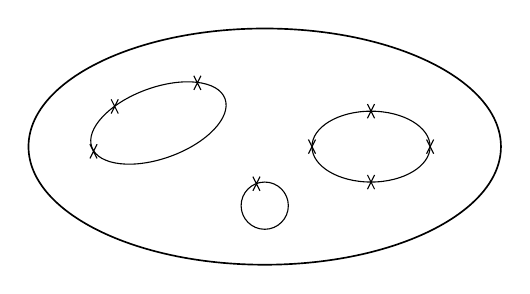
\begin{tikzpicture}[scale=1.5]
            \draw [semithick] ellipse (2cm and 1cm);
    
            \draw [rotate around={20:(-0.9,0.2)}] (-0.9,0.2) ellipse (6mm and 3mm);
            \draw (0,-0.5) circle (2mm);
            \draw (0.9,0) ellipse (5mm and 3mm);
    
            \draw [xshift=-1.48cm,yshift=-0.1cm,scale=0.6] (0,0) -- ++(0.1,0.2) ++(-0.1,0) -- ++(0.1,-0.2);
            \draw [xshift=-1.3cm,yshift=0.28cm,scale=0.6] (0,0) -- ++(0.1,0.2) ++(-0.1,0) -- ++(0.1,-0.2);
            \draw [xshift=-0.6cm,yshift=0.48cm,scale=0.6] (0,0) -- ++(0.1,0.2) ++(-0.1,0) -- ++(0.1,-0.2);
    
            \draw [xshift=-0.1cm,yshift=-0.374cm,scale=0.6] (0,0) -- ++(0.1,0.2) ++(-0.1,0) -- ++(0.1,-0.2);
    
            \draw [xshift=1.4cm,yshift=0cm,scale=0.3] (0,0) ++(-0.1,-0.2) -- ++(0.2,0.4) ++(-0.2,0) -- ++(0.2,-0.4);
            \draw [xshift=0.4cm,yshift=0cm,scale=0.3] (0,0) ++(-0.1,-0.2) -- ++(0.2,0.4) ++(-0.2,0) -- ++(0.2,-0.4);
            \draw [xshift=0.9cm,yshift=0.3cm,scale=0.3] (0,0) ++(-0.1,-0.2) -- ++(0.2,0.4) ++(-0.2,0) -- ++(0.2,-0.4);
            \draw [xshift=0.9cm,yshift=-0.3cm,scale=0.3] (0,0) ++(-0.1,-0.2) -- ++(0.2,0.4) ++(-0.2,0) -- ++(0.2,-0.4);
        \end{tikzpicture}
        \caption{Decomposing $\sigma$ into disjoint cycles.}
        \label{fig:disjointCycles}
    \end{figure}
    \begin{itemize}
        \item The idea behind this proposition is that every element will cycle back to itself eventually, and you can't get to elements of one cycle if you're not in the cycle (so all cycles are disjoint).
        \item Every permutation can be visualized by ordering the $n$ letters in a set in $\R^2$ and connecting all disjoint cycles (think a circle full of oriented circles/loops/cycles).
    \end{itemize}
    \item Composing cycles. See what the right one does and then the left one. Canonically, start with 1.
    \item Proposition: The cycle decomposition of $\sigma$ is unique up to\dots
    \begin{itemize}
        \item The ordering of the disjoint cycles;
        \item Cycle permutations of each cycle;
        \item Include/exclude 1-cycles.
    \end{itemize}
    Moreover, $|\sigma|$ is the least common multiple of the cycle lengths.
    \item How many elements in $S_6$ have a cycle shape that looks like $(x,x)(x,x)(x,x)$?
    \begin{itemize}
        \item It is
        \begin{equation*}
            \frac{6!}{2^3\cdot 3!} = 15
        \end{equation*}
        \item Rationale: See PSet 2, Q1a.
    \end{itemize}
    \item The cycle decompositions of all elements in $S_4$.
    \begin{table}[H]
        \centering
        \small
        \renewcommand{\arraystretch}{1.2}
        \begin{tabular}{|c|c|c|c|c|}
            $(1,2,3,4)$ & $(1,2,3)$ & $(1,2)$ & $(1,2)(3,4)$ & $e$\\
            $(1,2,4,3)$ & $(1,3,2)$ & $(1,3)$ & $(1,3)(2,4)$ &    \\
            $(1,3,2,4)$ & $(1,2,4)$ & $(1,4)$ & $(1,4)(2,3)$ &    \\
            $(1,3,4,2)$ & $(1,4,2)$ & $(2,3)$ &              &    \\
            $(1,4,2,3)$ & $(1,3,4)$ & $(2,4)$ &              &    \\
            $(1,4,3,2)$ & $(1,4,3)$ &         &              &    \\
                        & $(2,3,4)$ &         &              &    \\
                        & $(2,4,3)$ &         &              &    \\
        \end{tabular}
        \caption{$S_4$ cycle decompositions.}
        \label{tab:S4Cycles}
    \end{table}
    \item \textbf{Conjugate} (elements $x,y$): Two elements $x,y\in G$ a group for which there exists $g\in G$ such that $y=g\cdot x\cdot g^{-1}$. \emph{Denoted by} $\bm{x\sim y}$.
    \item Lemma: Conjugacy is an equivalence relation.
    \begin{enumerate}[label={(\Roman*)}]
        \item $x\sim x$.
        \begin{proof}
            $x=exe^{-1}$.
        \end{proof}
        \item If $y\sim x$, then $x\sim y$.
        \begin{proof}
            Take
            \begin{align*}
                y &= gxg^{-1}\\
                g^{-1}y(g^{-1})^{-1} &= x
            \end{align*}
        \end{proof}
        \item If $x\sim y$ and $y\sim z$, then $x\sim z$.
        \begin{proof}
            Suppose $y=gxg^{-1}$ and $z=hyh^{-1}$. Then
            \begin{equation*}
                z = hgxg^{-1}h^{-1}
                = (hg)x(hg)^{-1}
            \end{equation*}
        \end{proof}
    \end{enumerate}
    \item \textbf{Conjugacy class} (of $x$): A subset of $G$ containing all $g\in G$ which are conjugate to a certain $x\in G$. \emph{Given by}
    \begin{equation*}
        \{g\in G\mid g\sim x\}
    \end{equation*}
    \item Straightforward: Not necessarily obvious, but there's nothing really tricky going on.
    \begin{itemize}
        \item The joke about the mathematician who says something is obvious, someone asks why?, he thinks for 20 minutes, and then says it's obvious.
    \end{itemize}
    \item Why is conjugacy important?
    \begin{itemize}
        \item In linear algebra, we've seen it with similar matrices.
        \begin{itemize}
            \item Same linear map in a different basis is the same as conjugating the matrix of the map in one basis with the change of basis matrix.
        \end{itemize}
        \item Conjugacy tells us that a set of objects are, in some way, the same.
    \end{itemize}
\end{itemize}



\section{Conjugacy}
\begin{itemize}
    \item \marginnote{10/7:}You can request one extension per quarter on homework (possibly more if you have a really good reason) for sickness, etc., no questions asked. Email your TA to secure this extension.
    \item Last time, we began covering conjugacy.
    \begin{itemize}
        \item Conjugacy classes.
        \item Conjugacy defines an equivalence relation on $G$.
        \item $G=\bigsqcup\text{conjugacy classes}$\footnote{$\bigsqcup$ denotes a \textbf{disjoint union}. Think of the \emph{disjoint} union of sets as a union of sets that happen to be disjoint, the same way a \emph{direct} sum of subspaces is a sum of subspaces that happen to be linearly independent.}.
    \end{itemize}
    \item More on conjugacy today.
    \item The conjugacy class of $e$ is $\{e\}$.
    \item If $y=gxg^{-1}$, then $y^k=gx^kg^{-1}$.
    \item Proposition: $y\sim x$ implies $|y|=|x|$.
    \begin{proof}
        Suppose $|y|=k$, i.e., $y^k=e$. By the above statement, we know that $y^k\sim x^k$. Since $y^k=e$, it follows that $e\sim x^k$. Thus, $x^k$ is in the conjugacy class of $e$. But since the conjugacy class of $e$ is $\{e\}$, this means that $x^k=e$, as desired.
    \end{proof}
    \item Conjugacy in $S_n$, $n\geq 2$.
    \begin{itemize}
        \item Each $x\in S^n$ has a cycle decomposition
        \begin{equation*}
            x = (a_1,\dots,a_k)(b_1,\dots,b_m)(c_1,\dots)\cdots
        \end{equation*}
        \item We want to investigate the properties of $gxg^{-1}$ for an arbitrary $g\in S_n$. Ideally, we'd like to express it in a form related to $x$.
        \item Trick: Apply $gxg^{-1}$ to $g(a_1)$. Then
        \begin{equation*}
            gxg^{-1}(g(a_1)) = gx(a_1)
            = g(a_2)
        \end{equation*}
        \item It follows by induction that
        \begin{equation*}
            gxg^{-1} = (g(a_1),\dots,g(a_k))(g(b_1),\dots,g(b_m))(g(c_1),\dots)\cdots
        \end{equation*}
        \item Now suppose that $m\neq g(a_i),g(b_j),g(c_k),\dots$. Then
        \begin{equation*}
            g^{-1}(m) \notin \{a_1,\dots,a_k,b_1,\dots,b_m,c_1,\dots\}
        \end{equation*}
        It follows since $x$ is the identity on such elements that $x(g^{-1}(m))=g^{-1}(m)$. Therefore, since all functions involved are bijections,
        \begin{equation*}
            [gxg^{-1}](m) = g[x(g^{-1}(m))] = g(g^{-1}(m)) = m
        \end{equation*}
        \item It follows that $gxg^{-1}$ has the same cycle \textbf{shape}.
    \end{itemize}
    \item \textbf{Shape} (of $g\in S_n$): The partition of $n$ given by the lengths of the cycles in the cycle decomposition of $g$ in decreasing order. \emph{Also known as} \textbf{cycle shape}.
    \begin{table}[H]
        \centering
        \small
        \renewcommand{\arraystretch}{1.2}
        \begin{tabular}{c|c|c|c|c}
            $S_4$ & 4-cycle & 3-cycle & Product of 2-cycles & 1-cycles\\
            \hline
            Cycle decomposition & $(x,x,x,x)$ & $(x,x,x)(x)$ & $(x,x)(x,x)$ & $(x)(x)(x)(x)$\\
            Shape & $4$ & $3+1$ & $2+2$ & $1+1+1+1$\\
        \end{tabular}
        \caption{Shape of elements in $S_4$.}
        \label{tab:shapeS4}
    \end{table}
    \item Claim: $x,y\in S_n$ are conjugate iff they have the same cycle shape.
    \begin{proof}
        We will do a proof by example that illustrates the idea of the generalized proof.\par
        Let
        \begin{align*}
            x &= (1,2,3)(4,5,6)(7,10)&
            y &= (2,3)(4,1,5)(6,9,10)
        \end{align*}
        Note that both have the same cycle shape: $3+3+2+1+1$. We now use a two-step process to define a $g$ such that $y=gxg^{-1}$.\par
        Step 1: Including 1-cycles, line both $x$ and $y$ up so they "match."
        \begingroup
        \small
        \renewcommand{\arraystretch}{1.2}
        \begin{equation*}
            \begin{NiceArray}{c|c@{}ccc@{}c@{}ccc@{}c@{}cc@{}c@{}c@{}c@{}c@{}c}
                x        & (&  1   &  2   &  3   &)(&  4   &  5   &  6   &)(&  7   &  10   &)(&  8   &)(&  9   &)\\
                \hline
                y        & (&  4   &  1   &  5   &)(&  6   &  9   &  10  &)(&  2   &  3    &)(&  7   &)(&  8   &)\\
                \hline
                gxg^{-1} & (& g(1) & g(2) & g(3) &)(& g(4) & g(5) & g(6) &)(& g(7) & g(10) &)(& g(8) &)(& g(9) &)\\
            \end{NiceArray}
        \end{equation*}
        \endgroup
        Step 2: We want $y=gxg^{-1}$. Thus, take $g$ to be the map which sends every entry in $gxg^{-1}$ to the entry of $y$ directly above it. For example, we want $g(1)=4$, $g(2)=1$, $g(3)=5$, \dots. Noting that $g(1)=4$, $g(4)=6$, $g(6)=10$, \dots, we realize that $g$ can actually be written as the following cycle.
        \begin{equation*}
            g = (1,4,6,10,3,5,9,8,7,2)
        \end{equation*}
    \end{proof}
    \item Follow ups.
    \begin{itemize}
        \item How many different $g$'s satisfy $y=gxg^{-1}$?
        \begin{itemize}
            \item Depends on the number of ways $y$ can be matched up with $x$.
            \item The above manner obviously works.
            \item However, we can rotate the elements in both 3-cycles three ways, and the elements of the 2-cycle two ways, so that's $3\cdot 3\cdot 2=18$ $g$'s right there.
            \item Additionally, we can swap the place of the 3-cycles and the 1-cycles entirely, so thats an additional $2\cdot 2$ times as many ways.
            \item All told, there are $3\cdot 3\cdot 2\cdot 2\cdot 2=72$ possible $g$'s.
            \item See HW2, Q1a for a treatment of an analogous problem.
        \end{itemize}
        \item Counting the size of conjugacy classes.
        \begin{itemize}
            \item Suppose $G$ is an abelian group. Then if $y=gxg^{-1}$, $y=gg^{-1}x=x$, so the size of the conjugacy class of any $x\in G$ is 1.
            \item For this reason, the elements of $\Z/n\Z$ and of $\text{SO}(2)$ are conjugate only to themselves.
            \item However, we get something different for $\text{O}(2)$. Here, we can prove that the conjugacy class of every rotation $r$ is $\{r,r^{-1}\}$, and that all reflections are in the same conjugacy class\footnote{This is fundamentally related to the structure of point groups in inorganic chemistry! Remember that in $C_{5v}$, for instance, $C_5,C_5^4$ are conjugate, $C_5^2,C_5^3$ are conjugate, and all reflections get lumped together.}.
            \begin{itemize}
                \item Let $r$ denote a rotation, and $s$ denote a reflection.
                \item Suppose $x=r$. Then
                \begin{align*}
                    e &= (sr)^2\\
                    &= srsr\\
                    r^{-1} &= srs\\
                    &= srs^{-1}
                \end{align*}
                where we have HW1, Q2d(i) to justify the first equality and the fact that every reflection is it's own inverse\footnote{Intuitively, applying any reflection twice yields the original object.} to justify the last equality.
                \item On the other hand, suppose $x=s$. Then if $r$ is any rotation,
                \begin{align*}
                    srsr &= e\\
                    rsr &= s^{-1}\\
                    rsrr^{-2} &= s^{-1}r^{-2}\\
                    rsr^{-1} &= sr'
                \end{align*}
                where $r'$ denotes $r^{-2}$ to express the main takeaway: that $s$ is conjugate to itself times any rotation (for $r'$ arbitrary, we may choose $r=(r')^2$). In other words, since all reflections are related by some rotation, all reflections are, indeed, in the same conjugacy class.
            \end{itemize}
        \end{itemize}
    \end{itemize}
    \item Generators of $S_n$, $n\geq 3$.
    \item Lemma: The set of 2-cycles generates $S_n$.
    \begin{proof}
        It only requires $n-1$ swaps between pairs of elements to get to any permutation. For example, to get to
        \begin{equation*}
            \begin{matrix}
                1\\
                2\\
                3\\
                4\\
            \end{matrix}
            \mapsto
            \begin{matrix}
                3\\
                4\\
                2\\
                1\\
            \end{matrix}
        \end{equation*}
        we can swap 1 and 3 (so $1\mapsto 3$), then 2 and 4 (so $2\mapsto 4$), then "3" and "4" (so $3\mapsto 2$ and $4\mapsto 1$). More graphically,
        \begin{figure}[H]
            \centering
            \begin{tikzpicture}
                \matrix (A) [matrix of math nodes,column sep=1cm] {
                    1 & 3 & 3 & 3\\
                    2 & 2 & 4 & 4\\
                    3 & 1 & 1 & 2\\
                    4 & 4 & 2 & 1\\
                };
            
                \draw
                    (A-1-1) -- (A-3-2) -- (A-3-3) -- (A-4-4)
                    (A-2-1) -- (A-2-2) -- (A-4-3) -- (A-3-4)
                    (A-3-1) -- (A-1-2) -- (A-1-3) -- (A-1-4)
                    (A-4-1) -- (A-4-2) -- (A-2-3) -- (A-2-4)
                ;
            \end{tikzpicture}
            \caption{Generating $S_n$ with 2-cycles.}
            \label{fig:SnGenerate2}
        \end{figure}
        The idea is we fix the first element and then work down the list.
    \end{proof}
    \item $S_n$ is also generated by
    \begin{align*}
        \{(1,2),(2,3),(3,4),\dots,(n-1,n)\}&&
        \{(1,2),(1,3),(1,4),\dots,(1,n)\}
    \end{align*}
    \begin{itemize}
        \item Both of these sets have cardinality $n-1$.
    \end{itemize}
    \item As we can see from the above\dots
    \begin{itemize}
        \item If we generate $S_n$ with all 2-cycles, the generator set has cardinality $\frac{n}{2}(n-1)$;
        \item If we generate $S_n$ with all elementary 2-cycles, the generator set has cardinality $n-1$.
    \end{itemize}
    \item But we can do even better: Let $\sigma=(1,2)$ and $\tau=(1,2,\dots,n)$. Then any
    \begin{equation*}
        (k,k+1) = \tau^{k-1}\sigma\tau^{-(k-1)}
    \end{equation*}
    \begin{itemize}
        \item Indeed, we can see that using the RHS above, $k\mapsto 1\mapsto 2\mapsto k+1$ and $k+1\mapsto 2\mapsto 1\mapsto k$. Every other element receives the identity treatment, as we can confirm.
    \end{itemize}
\end{itemize}




\end{document}